\subsubsection{Flowchart}

\begin{figure}[H]
    \centerline{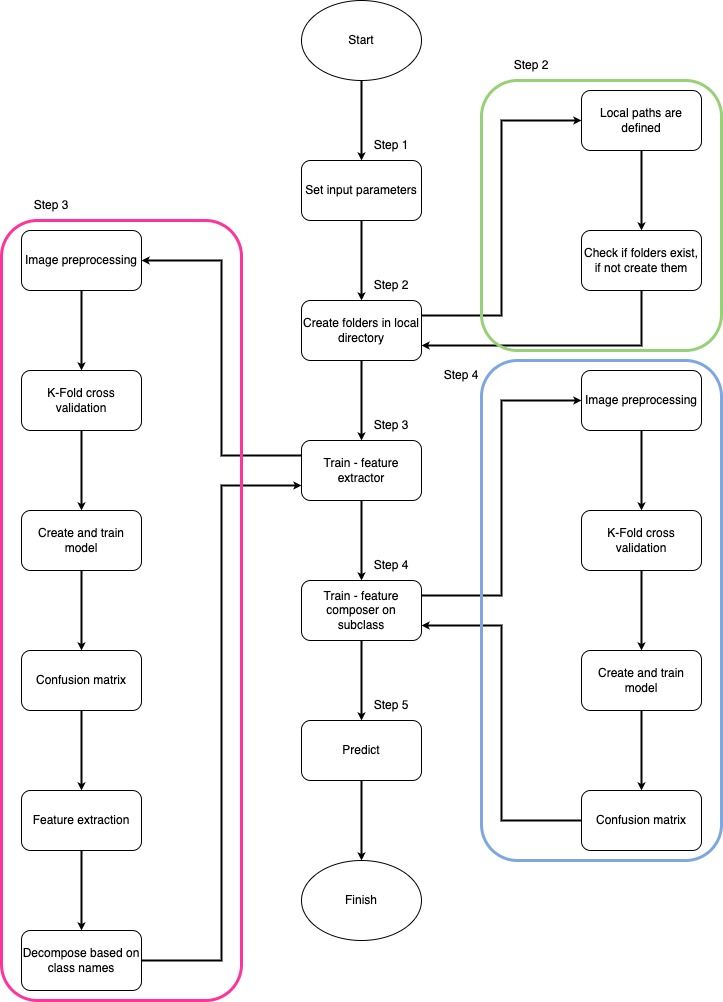
\includegraphics[scale=0.552]{img/DeTraCDiagram.jpg}}
    \caption{Figure representing flowchart of the code}
\end{figure}

The figure above is describing the steps that are taking place in order to have a successful program. If we have a look at the program from general perspective, we can deduct it into the 5 different steps. With this flowchart, we can go across each step and see where problem did occur and why. 

\begin{table}[!ht]
  \centering
    \begin{tabular}{ |m{12em}|m{20em}| } 
     \hline
        Step name & Step description \\ 
     \hline
        Step 1 & Configuration of parameters \\ 
     \hline
        Step 2 & Folders are created if they do not exist \\
     \hline
        Step 3 & Train the model on feature extractor \\
     \hline
        Step 4 & Train the model on composed or initial data\\
     \hline
        Step 5 & Model prediction\\
     \hline
    \end{tabular}
\caption{Description of steps in flowchart}
\end{table}